% \iffalse
%<*driver>
\input mydocstrip
\mygenerate[output-files/example-files/itemization]{
  example-asciilist-1.tex,
  example-asciilist-2.tex,
  example-easylist.tex,
  example-iitem.tex,
  example-philex.tex,
  example-wiki.tex,
}
\mygenerate[output-files/example-files/multi-file-projects]{
  % example-childdoc-1-main.tex,
  % example-childdoc-1-child.tex,
  % example-childdoc-2-main.tex,
  % example-childdoc-2-child.tex,
  % example-childdoc-3-main.tex,
}
\mygenerate[output-files/example-files/multi-file-projects/subfiles]{
  % example-childdoc-3-child.tex,
}
% \myendbatchfile
\documentclass[
  show-notes,
]{mydtxfile}
\usepackage{asciilist,iitem,wiki}
\usepackage[at]{easylist}
\NewDocumentCommand{\inputexample}{ m }{
% ^^A \tcolorbox[% \tcolorboxだと変になる
  \begin{tcolorbox}[
    colframe=black,
    fonttitle=\ttfamily\bfseries\large,
    title=#1,
  ]
  \input{output-files/example-files/#1}
% ^^A \endtcolorbox% \tcolorboxだと変になる
  \end{tcolorbox}
}
\begin{document}
\DocInput{\jobname.dtx}
\end{document}
%</driver>
% \fi
%
% \mytitle{Comparison of Packages for \LaTeX}
%
% \begin{concealableitemize}^^A [[[
% \1 The origin of title
%   \2 \doublequotes{TikZ is not the only graphics package for \TeX.}
%     \3 \texdoc[section=1.2 Comparison with Other Graphics Packages]{tikz}
%   \2 \doublequotes{I try to give a reasonably fair comparison of TikZ and other packages.}
%     \3 \texdoc[section=1.2 Comparison with Other Graphics Packages]{tikz}
% \end{concealableitemize}^^A ]]]
%
% \begin{abstract}^^A [[[
% このファイルはサイズが大きくなるがsubfilesに分けることはしない.
% なぜなら,そこまで頻繁に編集することはないと思うから.
%
% \begin{concealableitemize}^^A [[[
% \1 author
%   \2 \verb|\author| \mycite[page=183]{dokushu-latex2e}
% \1 conclusion
%   \2 
% \end{concealableitemize}^^A ]]]
%
% \end{abstract}^^A ]]]
%
% \begin{mynote}^^A [[[
% \begin{myitemize}
% \1 \verb|subcaption|は従来の\verb|subfigure|,\verb|subfig|を置き換える新しいパッケージである\cite[161]{latex2e-bibunshosakusei}.
% \1 captionのカスタマイズ.\href{http://konoyonohana.blog.fc2.com/blog-entry-264.html}{ここ}を参照.
% \1 
% \end{myitemize}
% \end{mynote}^^A ]]]
%
% \mytableofcontents[depth=3]
%
% \section{Attach files}^^A [[[
%
% \begin{concealableitemize}^^A [[[
% \1 The origin of `attach files'
%   \2 未確認
% \end{concealableitemize}^^A ]]]
%
% \subsection{Notes}^^A [[[
% \begin{myitemize}
% \1 attachfile
% \1 hypdvips
% \1 
% \end{myitemize}
% ^^A ]]] End of subsection `Notes'.
%
% \subsection{各Packageの詳細}^^A [[[
%
% \subsubsection{attachfile}^^A [[[
% \begin{myitemize}
% \1 Abstract
%   \2 
% \1 Author
%   \2 
% \1 References
%   \2 
% \1 Conclusion
% \end{myitemize}
%
% \begin{latexcode}
%<*example-attachfile.tex>



%</example-attachfile.tex>
% \end{latexcode}
% ^^A ]]] End of subsubsection `attachfile'.
%
% \subsubsection{hypdvips}^^A [[[
% \begin{myitemize}
% \1 Abstract
%   \2 
% \1 Author
%   \2 
% \1 References
%   \2 
% \1 Conclusion
% \end{myitemize}
%
% \begin{latexcode}
%<*example-hypdvips.tex>

%</example-hypdvips.tex>
% \end{latexcode}
% ^^A ]]] End of subsubsection `hypdvips'.
%
% ^^A ]]] End of subsection `Package'.
%
% \subsection{Conclusion}^^A [[[
%
%
%
%
% ^^A ]]] End of subsection `Conclusion'.
%
% ^^A ]]] End of section `Attach files'.
%
% \endinput
%
% \section{Presentation slides}^^A [[[
%
% \begin{concealableitemize}^^A [[[
% \1 The origin of `presentation slides'
%   \2 Beamer is a LaTeX document class for creating presentation slides,
%   with a wide range of templates and a set of features for making slideshow effects
%   \mycite[keyword=Beamer (LaTeX)]{wikipedia}
%   \2 
% \end{concealableitemize}^^A ]]]
%
% \subsection{Notes}^^A [[[
% \begin{myitemize}
% \1 The Beamer class is not the first LaTeX class for creating presentations,
% and like many of its predecessors (such as \verb|slides|, \verb|seminar|, \verb|prosper|, \verb|powerdot|),
% it has special syntax for defining "slides" (known in Beamer as "frames")
% \mycite[keyword=Beamer (LaTeX), section=Method]{wikipedia}.
% \1 \href{https://tex.stackexchange.com/questions/16204/which-package-to-use-for-presentations-beamer-prosper-or-other}{Which package to use for presentations? Beamer, Prosper, or Other}
% \1 
% \1 
% \end{myitemize}
% ^^A ]]] End of subsection `Notes'.
%
% \subsection{各Packageの詳細}^^A [[[
%
% \subsubsection{beamer}^^A [[[
% \begin{myitemize}
% \1 Abstract
%   \2 
% \1 Author
%   \2 
% \1 References
%   \2 
% \1 Conclusion
% \end{myitemize}
% ^^A ]]] End of subsubsection `beamer'.
%
% \subsubsection{powerdot}^^A [[[
% \begin{myitemize}
% \1 Abstract
%   \2 
% \1 Author
%   \2 
% \1 References
%   \2 
% \1 Conclusion
% \end{myitemize}
%
% \begin{latexcode}
%<*example-wiki.tex>
\wikiEnvironments
# One
# Two
This a normal paragraph
* One
* Two
* Three
Another normal paragraph
;[One description] Lorem ipsum dolor sit amet, consectetuer adipiscing elit, sed diam nonummy nibh euismod tincidunt ut laoreet dolore magna aliquam erat volutpat.
;[Another] Lorem ipsum dolor sit amet, consectetuer adipiscing elit, sed diam nonummy nibh euismod tincidunt ut laoreet dolore magna aliquam erat volutpat.
\nowikiEnvironments
%</example-wiki.tex>
% \end{latexcode}
% ^^A ]]] End of subsubsection `***'.
%
% \subsubsection{prosper}^^A [[[
% \begin{myitemize}
% \1 Abstract
%   \2 
% \1 Author
%   \2 
% \1 References
%   \2 
% \1 Conclusion
% \end{myitemize}
% ^^A ]]] End of subsubsection `prosper'.
%
% \subsubsection{seminar}^^A [[[
% \begin{myitemize}
% \1 Abstract
%   \2 
% \1 Author
%   \2 
% \1 References
%   \2 
% \1 Conclusion
% \end{myitemize}
% ^^A ]]] End of subsubsection `seminar'.
%
% \subsubsection{slides}^^A [[[
% \begin{myitemize}
% \1 Abstract
%   \2 
% \1 Author
%   \2 
% \1 References
%   \2 
% \1 Conclusion
% \end{myitemize}
%
% \begin{latexcode}
%<*example-wiki.tex>
\wikiEnvironments
# One
# Two
This a normal paragraph
* One
* Two
* Three
Another normal paragraph
;[One description] Lorem ipsum dolor sit amet, consectetuer adipiscing elit, sed diam nonummy nibh euismod tincidunt ut laoreet dolore magna aliquam erat volutpat.
;[Another] Lorem ipsum dolor sit amet, consectetuer adipiscing elit, sed diam nonummy nibh euismod tincidunt ut laoreet dolore magna aliquam erat volutpat.
\nowikiEnvironments
%</example-wiki.tex>
% \end{latexcode}
% ^^A ]]] End of subsubsection `slides'.
%
% ^^A ]]] End of subsection `Package'.
%
% \subsection{Conclusion}^^A [[[
%
%
%
%
% ^^A ]]] End of subsection `Conclusion'.
%
% ^^A ]]] End of section `Presentation slides'.
%
% \section{Itemization}^^A [[[
%
% \begin{concealableitemize}^^A [[[
% \1 The origin of `itemization'
%   \2 \href{https://eikaiwa.dmm.com/uknow/questions/76527/}{箇条書きって英語でなんて言うの?}
%   \2 \mycite[keyword=箇条書き]{weblio}
% \end{concealableitemize}^^A ]]]
%
% \subsection{Notes}^^A [[[
% \begin{myitemize}
% \1 \texdoc[section=5 Related Packages]{asciilist}に箇条書き関係のパッケージがまとめられている
% \1 \href{http://konoyonohana.blog.fc2.com/blog-entry-415.html}{[LaTeX] 最新版:公開済みパッケージ一覧表(目的別順)}
% \1 \href{https://tex.stackexchange.com/questions/150865/simplify-itemize-commands-typesetting}
% {Simplify itemize commands typesetting}
% \1 
% \end{myitemize}
%
% \begin{mynote}^^A [[[
% \verb|enumitem|パッケージは箇条書きの体裁を変えるだけのパッケージ
% \end{mynote}^^A ]]]
%
% ^^A ]]] End of subsection `Notes'.
%
% \subsection{各Packageの詳細}^^A [[[
%
% \subsubsection{asciilist}[updated=2021-07-11T15:06:21]^^A [[[
% \begin{myitemize}
% \1 Abstract
%   \2 アスキー文字でlevelを指定できる
% \1 Author
%   \2 Richard Grewe
% \1 Conclusion
%   \2 不備が多々存在する
% \end{myitemize}
%
% \paragraph{Example 1 (Indentation問題)}[updated=2021-07-11T15:05:30]^^A [[[
% 次のように,\verb|\end{AsciiList}|の直後がインデントされてしまう:
% ^^A 以下のEulerについての参照先:\url{https://en.wikipedia.org/wiki/Euler_integral}
% \begin{latexcode}
%<*example-asciilist-1.tex>
\noindent Eulerの業績:
\begin{AsciiList}{-,*,+,=}
- Euler's formula
  * $e^{ix}=\cos x+i\sin x$
- Euler integral
  * Euler integral of the first kind: the beta function
  * Euler integral of the second kind: the gamma function
\end{AsciiList}
など.
ここで$\displaystyle B(x,y)=\int_0^1t^{x-1}(1-t)^{y-1}dt$,
$\displaystyle\Gamma(z)=\int_0^\infty t^{z-1}e^{-t}dt$である.
For positive integers $n$, $\Gamma(n)=(n-1)!$.
%</example-asciilist-1.tex>
% \end{latexcode}
%
% ^^A \inputexample{example-asciilist-1.tex} \inputexampleで表示するとインデントされない
% \verb|example-asciilist-1.tex|の出力
% \footnote{%
%   \texcommand{inputexample}で表示するとインデントされないので,
%   \texcommand{input}で表示する.
% }:\\
% -----------------------------------------------------------\\
% \input{output-files/example-files/itemization/example-asciilist-1}
% \noindent-----------------------------------------------------------
% ^^A ]]] End of paragraph `Example 1'.
%
% \paragraph{Example 2 (New line問題)}[updated=2021-07-11T15:05:43]^^A [[[
% 途中で改行するとスペースが入ってしまう:
% \begin{latexcode}
%<*example-asciilist-2.tex>
\begin{AsciiList}{-,*,+,=}
- 吾輩は
猫である.
\end{AsciiList}
%</example-asciilist-2.tex>
% \end{latexcode}
%
% \inputexample{itemization/example-asciilist-2.tex}
% ^^A ]]] End of paragraph `Example 2'.
%
% \paragraph{Example 3 (Footnote問題)}[updated=2020-05-16T08:37:14]^^A [[[
% 次のコードはなぜかエラーになってしまう:
% \begin{latexcode}
%<*example-asciilist-3.tex>
\documentclass{ltjsarticle}
\usepackage{asciilist}
\begin{document}
\begin{AsciiList}{-,*,+,=}
- 吾輩は猫\footnote{%
  cat
} である.
\end{AsciiList}
\end{document}
%</example-asciilist-3.tex>
% \end{latexcode}
% ^^A ]]] End of paragraph `Example 3'.
%
% ^^A ]]] End of subsubsection `asciilist'.
%
% \subsubsection{cjwoutl}[updated=2021-07-11T15:13:08]^^A [[[
% \begin{myitemize}
% \1 Abstract
%   \2 相対的にlevelを指定できる.
% \1 Conclusion
%   \2 入力文字数が多くなるデメリットあり
%   \2 標準でインストールされない
%     \3 \bashinline{sudo apt install texlive-full}でもインストールされない
% \end{myitemize}
%
% サンプル\urlref{http://konoyonohana.blog.fc2.com/blog-entry-284.html}{%
%   [LaTeX] cjwoutl --- enumerateのようなアウトライン環境%
% }:
% \begin{latexcode}
%<*example-cjwoutl.tex>
\documentclass{ltjsarticle}
\usepackage{cjwoutl}
\begin{document}
Example
\begin{outline}
\outl{1} top level
  \outl{+} down level
  \outl{=} same level
\outl{-} up level
\end{outline}
Itemize
\end{document}
%</example-cjwoutl.tex>
% \end{latexcode}
% ^^A ]]] End of subsubsection `cjwoutl'.
%
% \subsubsection{easylist}[updated=2021-07-11T15:27:08]^^A [[[
% \begin{myitemize}
% \1 Abstract
%   \2 文字数でlevelを指定できる
% \1 Author
%   \2 Paul Isambert
% \1 Conclusion
%   \2 Footnote問題なし
%   \2 New line問題なし
%   \2 Indentation問題あり
%   \2 levelに応じて入力文字数が増えるデメリットあり
% \end{myitemize}
%
% \paragraph{Example 1 (@問題)}[updated=2021-07-11T15:26:48]^^A [[[
% easylist環境内で普通には\verb|@|を使えない問題あり.
% 次のコードだと\verb|sample@gmail.com|の\verb|@|が表示されない.
% \begin{latexcode}
%<*example-easylist.tex>
\noindent 例えば,
\begin{easylist}[itemize]
@ 吾輩は猫\footnote{%
  cat
} である.
@ 芥川龍之介
  @@ 人間失格を
  読む.
  @@ sample@gmail.com
\end{easylist}
インデント問題あり.sample@gmail.com
%</example-easylist.tex>
% \end{latexcode}
%
% ^^A \inputexample{example-easylist.tex} \inputexampleで表示するとインデントされない
% \verb|example-easylist.tex|の出力
% \footnote{%
%   \texcommand{inputexample}で表示するとインデントされないので,
%   \texcommand{input}で表示する.
% }:\\
% -----------------------------------------------------------\\
% \input{output-files/example-files/itemization/example-easylist}
% \noindent-----------------------------------------------------------
% ^^A ]]] End of paragraph `Example 1'.
%
% ^^A ]]] End of subsubsection `easylist'.
%
% \subsubsection{iitem}[updated=2021-07-11T15:51:35]^^A [[[
% \begin{myitemize}
% \1 Abstract
%   \2 \verb|\iitem|,\verb|\iiitem|など\verb|i|の文字数でlevelを変える
% \1 Author
%   \2 Ben Vitecek
% \1 Conclusion
%   \2 Indentation問題なし
%   \2 Footnote問題なし
%   \2 New line問題あり(改行されてしまう)
%   \2 入力文字数が他のパッケージと比べて多くなるデメリットがある.
%     \3 ただ,\verb|\newcommand{\2}{\iitem}|でその点は解決するが...
% \end{myitemize}
%
% \begin{latexcode}
%<*example-iitem.tex>
\noindent Eulerの業績:
\begin{itemize}
\item Euler's formula
  \iitem $e^{ix}=\cos x+i\sin x$
\item Euler integral
  \iitem Euler integral of the first kind:
  the beta function
  \iitem Euler integral of the second kind: the gamma function\footnote{%
    $\displaystyle\Gamma(z)=\int_0^\infty t^{z-1}e^{-t}dt$
  }
\end{itemize}
など.
%</example-iitem.tex>
% \end{latexcode}
%
% ^^A \inputexample{example-iitem.tex} \inputexampleで表示するとインデントされない
% \verb|example-iitem.tex|の出力
% \footnote{%
%   \texcommand{inputexample}で表示するとインデントされないので,
%   \texcommand{input}で表示する.
% }:\\
% -----------------------------------------------------------\\
% \input{output-files/example-files/itemization/example-iitem}
% \noindent-----------------------------------------------------------
% ^^A ]]] End of subsubsection `iitem'.
%
% \subsubsection{linguex}^^A [[[
% \begin{myitemize}
% \1 Abstract
%   \2 コマンドのみでenumitem環境を出力できる
% \1 Conclusion
%   \2 エンハンス版\verb|philex|パッケージがあるので却下
% \end{myitemize}
%
% \href{http://konoyonohana.blog.fc2.com/blog-entry-162.html}{ここ}を参照せよ.
%
% 箇条書きにするには\verb|\ex.[\hfill$\bullet$\hfill]|とする\texdoc[section=Customizing Labels]{linguex}.
%
% 空行でenumerate終了.
% 終了するために空行を入れる必要があるのはマイナス.
%
% \begin{latexcode}
%<*example-linguex.tex>
\documentclass{ltjsarticle}
\usepackage{linguex}
\begin{document}
\noindent Eulerの業績:
\ex.[\hfill$\bullet$\hfill] Euler's formula

\ex.[\hfill$\bullet$\hfill] Euler integral
  \a.[\hfill---\hfill] Euler integral of the first kind: the beta function
  \b.[\hfill---\hfill] Euler integral of the second kind: the gamma function

など.
\end{document}
%</example-linguex.tex>
% \end{latexcode}
% ^^A ]]] End of subsubsection `linguex'.
%
% \subsubsection{outlines}[updated=2021-07-11T15:58:02]^^A [[[
% \begin{myitemize}
% \1 Abstract
%   \2 \verb|\1|,\verb|\2|,\verb|\3|でlevelを変更できる(\verb|\0|もある)
% \1 Author
%   \2 Charles Pecheur
% \1 Conclusion
%   \2 Indentation問題なし
%   \2 New line問題なし
%   \2 Footnote問題なし
%   \2 入力文字数も少なくて済む(\verb|\1|,\verb|\2|,など)
% \end{myitemize}
% ^^A ]]] End of subsubssection `outlines'.
%
% \subsubsection{philex}^^A [[[
% \begin{myitemize}
% \1 Abstract
%   \2 The package is a small addition to Wolfgang Sternefeld's \verb|linguex| package
%   and requires \verb|linguex| \texdoc[section=Manual]{philex}.
% \1 Author
%   \2 Peter Pagin
% \1 Conclusion
% \end{myitemize}
% コマンドのみでenumitem環境を出力できる.
% 相互参照するときに便利そう
%
% いちいちラベルを指定するのは煩わしい.
%
% ただ,相互参照が必要になる場合は使えそう.
% \begin{latexcode}
%<*example-philex.tex>
\documentclass{ltjsarticle}
\usepackage{linguex}
\begin{document}
\noindent Eulerの業績:
\lb{label1}{Euler's formula
  \lba{label1-1} $e^{ix}=\cos x+i\sin x$
}
\lb{label2}{Euler integral
  \lba{label2-1} Euler integral of the first kind: the beta function
  \lba{label2-2} Euler integral of the second kind: the gamma function
}
など.
\rf{label1-1}からEulerの等式が得られる.
\end{document}
%</example-philex.tex>
% \end{latexcode}
% ^^A ]]] End of subsubsection `philex'.
%
% \subsubsection{wiki}^^A [[[
% \begin{myitemize}
% \1 Abstract
%   \2 
% \1 Author
%   \2 
% \1 References
%   \2 \href{https://tex.stackexchange.com/questions/150865/simplify-itemize-commands-typesetting}
%   {Simplify itemize commands typesetting}
%   \2 \href{https://anorien.csc.warwick.ac.uk/mirrors/CTAN/macros/latex/contrib/nicetext/doc/wikicheat.pdf}{wikicheat.pdf}
% \1 Conclusion
% \end{myitemize}
%
% \begin{latexcode}
%<*example-wiki.tex>
\wikiEnvironments
# One
# Two
This a normal paragraph
* One
* Two
* Three
Another normal paragraph
;[One description] Lorem ipsum dolor sit amet, consectetuer adipiscing elit, sed diam nonummy nibh euismod tincidunt ut laoreet dolore magna aliquam erat volutpat.
;[Another] Lorem ipsum dolor sit amet, consectetuer adipiscing elit, sed diam nonummy nibh euismod tincidunt ut laoreet dolore magna aliquam erat volutpat.
\nowikiEnvironments
%</example-wiki.tex>
% \end{latexcode}
%
% ^^A \inputexample{example-iitem.tex} \inputexampleで表示するとインデントされない
% \verb|example-wiki.tex|の出力
% \footnote{%
%   \texcommand{inputexample}で表示するとインデントされないので,
%   \texcommand{input}で表示する.
% }:\\
% -----------------------------------------------------------\\
% \input{output-files/example-files/itemization/example-wiki}
% \noindent-----------------------------------------------------------
% ^^A ]]] End of subsubsection `wiki'.
%
% ^^A ]]] End of subsection `Package'.
%
% \subsection{Conclusion}^^A [[[
% 入力文字数が増えることについては,問題としない.
% 理由は,例えば\verb|\newcommand{\2}{\iitem}|と再定義すれば解決するため.
%
% \renewcommand{\temporarycommand}[5]{#1&#2&#3&#4&#5\\}
% \begin{mytabular}{lllll}
% \temporarycommand{Package}  {Indentation問題}{Footnote問題}  {New line問題}  {Install問題} \hline
% \temporarycommand{asciilist}{yes}            {yes}           {yes}           {no}
% \temporarycommand{cjwoutl}  {uninvestigated} {uninvestigated}{uninvestigated}{yes}
% \temporarycommand{easylist} {yes}            {no}            {no}            {no}
% \temporarycommand{iitem}    {yes}            {no}            {no}            {no}
% \temporarycommand{outlines} {no}             {no}            {no}            {no}
% \end{mytabular}
%
% \doublequotes{uninvestigated} \mycite[keyword=未調査]{weblio}.
%
% \begin{mytip}[title=Conclusion]^^A [[[
% \verb|outlines|パッケージを使うことにする
% \end{mytip}^^A ]]]
%
% ^^A ]]] End of subsection `Conclusion'.
%
% ^^A ]]] End of section `Itemization'.
%
% \section{Multi-file projects}^^A [[[
%
% \begin{concealableitemize}^^A [[[
% \1 The origin of \verb|multi-file-projects|
%   \2 \texdoc[section=A Document Class and a Package for Handling Multi-File Projects]{subfiles}
% \end{concealableitemize}^^A ]]]
%
% \subsection{Notes}^^A [[[
% 関連パッケージについて比較・言及されている記事:
% \begin{myitemize}
% \1 \texdoc[section=1 Introduction]{docmute}
% \1 \texdoc[section=4.3 Similar packages and classes]{standalone}
% \1 \texdoc[section=3.3 Related CTAN Packages]{childdoc}
% \1\href{https://ctan.org/topic/subdocs}{subdocs}
% \end{myitemize}
%
% \begin{myitemize}
% \1 docmute
% \1 includeRnw
%   \2 This package is for including \verb|.Rnw|-files in normal \verb|.tex|-files \texdoc{includeRnw}.
%   \2 \href{https://ctan.org/topic/subdocs}{Include .Rnw inside .tex.}
% \1 includex
%   \2 This package is useful but may have problems and is unsupported \texdoc[section=Abstract]{includex}.
% \1 minidocument
%   \2 \href{https://ctan.org/topic/subdocs}{Creates miniature documents inside other LATEX documents.}
%   \2 
% \1 newclude
%   \2 \href{https://ctan.org/topic/subdocs}{Reimplemented include system for LATEX.}
%   \2 
% \1 standalone
%   \2 \url{https://www.overleaf.com/learn/latex/Multi-file_LaTeX_projects#The_standalone_package}
%   \2 However, the class class will import the preamble from a given main file,
%   while standalone is designed more for the opposite direction
%   where the preamble of subfiles can be imported to the main document
%   \texdoc[section=4.3 Similar packages and classes]{standalone}.
%   \2 
% \1 subdocs
%   \2 This is an experimental package aiming to provide a different approach for multidocument works
%   \urlref{https://ctan.org/pkg/subdocs?lang=en}{subdocs – Multifile documents}.
%   \2 The present release is an \emph{alpha version}
%   \urlref{https://ctan.org/pkg/subdocs?lang=en}{subdocs – Multifile documents}.
% \1 subfiles
%   \2 
% \end{myitemize}
% ^^A ]]] End of subsection `Notes'.
%
% \subsection{各Packageの詳細}^^A [[[
%
% \subsubsection{childdoc}^^A [[[
% \begin{myitemize}
% \1 Abstract
%   \2 \verb|childdoc| is a \LaTeXe{} package that enables the direct compilation of document sections
%   included by \verb|\include| to individual files \texdoc[section=Abstract]{childdoc}.
%   \2 \verb|\input{childdoc.def}|,\verb|\childdocmain{}|,\verb|\childdocof{main}|などを
%   書くことにより,コンパイル可能にする.
% \1 Author
%   \2 Niklas Beisert
% \1 Conclusion
%   \2 Preamble問題
%   \2 Subdirectory問題
% \end{myitemize}
%
% Subdirectories and special characters should be avoided in filenames
% \texdoc[section= 2.1 Included Files]{childdoc}.
% すなわち,\verb|\childdocof{../main-file}|のようにはできない.
%
% \paragraph{Example 1 (Basic usage)}[updated=2021-07-11T21:33:13]^^A [[[
%
% \begin{concealableitemize}^^A [[[
% \1 The origin of `basic usage'
%   \2 \texdoc[section=3 Basic usage]{minted}
%   \2 \texdoc[section=5.1 Basic usage]{standalone}
%   \2 \texdoc[section=2 Basic usage]{subfiles}
% \end{concealableitemize}^^A ]]]
%
% \begin{myitemize}
% \1 References
%   \2 \texdoc[section=2.1 Included Files]{childdoc}
%   \2 \href{https://konoyonohana.blog.fc2.com/blog-entry-396.html}
%   {[LaTeX] childdoc --- \texcommand{include}された子ドキュメントも直接コンパイルする}
% \end{myitemize}
%
% \begin{latexcode}
%<*example-childdoc-1-main.tex>
\input{childdoc.def}
\childdocmain{}
\documentclass{ltjsarticle}
\begin{document}
\include{example-childdoc-1-child}
\section{Second Section}
\end{document}
%</example-childdoc-1-main.tex>
% \end{latexcode}
%
% \begin{latexcode}
%<*example-childdoc-1-child.tex>
\input{childdoc.def}
\childdocof{example-childdoc-1-main}
\section{First Section}
Einstein's famous formula:
\[
  E=mc^2
\]
%</example-childdoc-1-child.tex>
% \end{latexcode}
% ^^A ]]] End of paragraph `Example 1 (Basic usage)'.
%
% \paragraph{Example 2 (Preamble問題)}[updated=]^^A [[[
% いけるっぽい****
% \begin{latexcode}
%<*example-childdoc-2-main.tex>
\input{childdoc.def}
\childdocmain{}
\documentclass{ltjsarticle}
\newcommand{\mycmd}[1]{\textsf{mycmd: #1}}
\begin{document}
\include{example-childdoc-2-child}
\section{Second Section}
\end{document}
%</example-childdoc-2-main.tex>
% \end{latexcode}
%
% \begin{latexcode}
%<*example-childdoc-2-child.tex>
\input{childdoc.def}
\childdocof{example-childdoc-2-main}
\section{First Section}
\mycmd{Cauchy}
\begin{itemize}
\item Cauchy distribution
\item Cauchy sequence
\item Cauchy–Schwarz inequality
\item Cauchy–Riemann equations
\item Cauchy's integral theorem
\end{itemize}
%</example-childdoc-2-child.tex>
% \end{latexcode}
% ^^A ]]] End of paragraph `Example 2'.
%
% \paragraph{Example 3 (Subdirectory問題)}[updated=]^^A [[[
% 上手く行かない???
% \begin{latexcode}
%<*example-childdoc-3-main.tex>
\input{childdoc.def}
\childdocmain{}
\documentclass{ltjsarticle}
\newcommand{\mycmd}[1]{\textsf{3: #1}}
\begin{document}
\include{subfiles/example-childdoc-3-child}
\section{Second Section}
\end{document}
%</example-childdoc-3-main.tex>
% \end{latexcode}
%
% \begin{latexcode}
%<*example-childdoc-3-child.tex>
\input{childdoc.def}
\childdocof{../example-childdoc-3-main}
\section{First Section}
\mycmd{Cauchy}
Riemann
%</example-childdoc-3-child.tex>
% \end{latexcode}
% ^^A ]]] End of paragraph `Example 3'.
%
% ^^A ]]] End of subsubsection `childdoc'.
%
% \subsubsection{combine}^^A [[[
% \begin{myitemize}
% \1 Abstract
%   \2 \verb|papers|環境の\verb|\import|で読み込むことでコンパイルを可能にする
% \1 Author
%   \2 Peter Wilson, Herries Press
% \1 Conclusion
%   \2 main fileに定義されたコマンドはsubfileでは使用できない
% \end{myitemize}
%
% \begin{latexcode}
%<*example-combine-main.tex>
\documentclass{combine}
\newcommand{\testcmd}{Test!!!}
\begin{document}
\begin{papers}
Sample document
\import{example-combine-child}
\section{Second Section}
Euler
\end{papers}
\end{document}
%</example-combine-main.tex>
% \end{latexcode}
%
% \begin{latexcode}
%<*example-combine-child.tex>
\documentclass{ltjsarticle}
\begin{document}
\section{First Section}
Einstein's famous formula:
\[
  E=mc^2
\]
\testcmd
\end{document}
%</example-combine-child.tex>
% \end{latexcode}
% ^^A ]]] End of subsubsection `combine'.
%
% \subsubsection{docmute}^^A [[[
% \begin{myitemize}
% \1 Abstract
%   \2 This package is intentionally kept simple.
%   If you require more smarts, there are other possibilities that might suit you better,
%   such as the \verb|standalone| package and document class by M. Scharrer
%   or the \verb|combine| class by W. Robertson and P. R. Wilson
%   \texdoc[section=1 Introduction]{docmute}.
%   \2 The package is loaded with the usual \verb|\usepackage{docmute}|.
%   It redefines the \verb|\documentclass| command in such a way that
%   everything between this command and the \verb|\begin{document}| is skipped,
%   as well as everything after the \verb|\end{document}|.
%   No attempts are made to analyse the actual content of the preamble---it is simply discarded
%   \texdoc[section=2 Usage]{docmute}.
% \1 Author
%   \2 Tomasz M. Trzeciak
% \1 Conclusion
%   \2 
% \end{myitemize}
%
% docmute ではプリアンブルの共有はサポートされていません.
% 個々の独立した LaTeX ファイルを include するのであれば docmute は良いかもしれませんが,
% 大規模な1つの LaTeX 文書を分割するのであれば,subfiles の方が便利です
% \urlref{https://qiita.com/sankichi92/items/1e113fcf6cc045eb64f7}{%
%   分割した LaTeX ファイルを subfiles を使ってコンパイルする%
% }.
%
% \begin{latexcode}
%<*example-docmute-main.tex>
\documentclass{ltjsarticle}
\usepackage{docmute}
\newcommand{\testcmd}{Test!!!}
\begin{document}
Test code
\input{example-docmute-sub}
\end{document}
%</example-docmute-main.tex>
% \end{latexcode}
%
% \begin{latexcode}
%<*example-docmute-sub.tex>
\documentclass{ltjsarticle}
\begin{document}
Test code 2
\[
  e^x=\sum_{n=0}^\infty\frac{x^n}{n!}
\]
\testcmd
\end{document}
%</example-docmute-sub.tex>
% \end{latexcode}
% ^^A ]]] End of subsubsection `docmute'.
%
% \subsubsection{standalone}^^A [[[
%
%    \begin{macrocode}
%<*example-standalone-main.tex>
\documentclass{ltjsarticle}
\usepackage{standalone}
\begin{document}
Test code
\input{example-standalone-sub}
\end{document}
%</example-standalone-main.tex>
%    \end{macrocode}
%
%    \begin{macrocode}
%<*example-standalone-sub.tex>
\documentclass{standalone}
\usepackage{standalone}
\newcommand{\testcmd}{Test!!!}
\begin{document}
\testcmd
\[
    \sin x=\sum_{n=0}^\infty\frac{(-1)^n}{(2n+1)!}x^{2n+1},\quad\cos x=\sum_{n=0}^\infty\frac{(-1)^n}{(2n)!}x^{2n}
\]
\end{document}
%</example-standalone-sub.tex>
%    \end{macrocode}
% ^^A ]]] End of subsubsection `standalone'.
%
% \subsubsection{subfiles}^^A [[[
%
% \paragraph{Example 1 (Basic usage)}[updated=]^^A [[[
% 以下のようにpreambleの共有もできる.
% \begin{latexcode}
%<*example-subfiles-main.tex>
\documentclass{ltjsarticle}
\newcommand{\testcmd}{Test!}
\usepackage{subfiles}
\begin{document}
Sample document
\subfile{example-subfiles-subfile}
\section{Second Section}
Euler
\end{document}
%</example-subfiles-main.tex>
% \end{latexcode}
%
% \begin{latexcode}
%<*example-subfiles-subfile.tex>
\documentclass[example-subfiles-main]{subfiles}
\begin{document}
\section{First Section}
\verb|subfiles| package \testcmd
\end{document}
%</example-subfiles-subfile.tex>
% \end{latexcode}
% ^^A ]]] End of paragraph `Example 1 (Basic usage)'.
%
% ^^A ]]] End of subsubsection `subfiles'.
%
% \subsubsection{}^^A [[[
%
% ^^A ]]] End of subsubsection `'.
%
% ^^A ]]] End of subsection `Package'.
%
% \subsection{Conclusion}^^A [[[
% \renewcommand{\temporarycommand}[5]{#1&#2&#3&#4&#5\\}
% \begin{mytabular}{lllll}
% \temporarycommand{package}  {Preamble共有問題}  {Subdirectory問題}  {問題}      {問題} \hline
% \temporarycommand{childdoc} {no}                {yes}               {yes}               {no}
% \temporarycommand{combine}  {yes}               {uninvestigated}               {yes}               {no}
% \temporarycommand{docmute}  {yes}               {uninvestigated}               {yes}               {no}
% \temporarycommand{subfiles} {no}                {no}                {}               {}
% \end{mytabular}
%
% \doublequotes{uninvestigated} \mycite[keyword=未調査]{weblio}.
%
% \verb|outlines|パッケージを使うことにする.
% ^^A ]]] End of subsection `Conclusion'.
%
% ^^A ]]] End of section `Multi-file projects'.
%
% \section{Graphics関係}^^A [[[
%
% \subsection{関連パッケージについて比較・言及されている記事}^^A [[[
% \begin{myitemize}
% \1 \texdoc[section=1.2 Comparison with Other Graphics Packages]{tikz}
% \1 
% \end{myitemize}
% ^^A ]]] End of subsection `***'.
%
% \subsection{各パッケージについて}^^A [[[
%
% \subsubsection{dratex}^^A [[[
% The \verb|dratex| package is a small graphic package for creating a graphics.
% Compared to the other package, including TikZ, it is very small, which may or may not be an advantage
% \texdoc[section=1.2 Comparison with Other Graphics Packages]{tikz}.
% ^^A ]]] End of subsubsection `dratex'.
%
% \subsubsection{metapost}^^A [[[
% The \verb|metapost| program is a powerful alternative to TikZ.
% It used to be an external program, which entailed a bunch of problems, but in Lua\TeX it is now build in.
% An obstacle with metapost is the inclusion of labels.
% This is much easier to achieve using pgf \texdoc[section=1.2 Comparison with Other Graphics Packages]{tikz}.
% ^^A ]]] End of subsubsection `metapost'.
%
% \subsubsection{pstricks}^^A [[[
% The \verb|pstricks| package is certainly powerful enough to create any conceivable kind of graphic,
% but it is not really portable.
% Most importantly, it does not work with \verb|pdftex| nor with any other driver
% that produces anything but PostScript code \texdoc[section=1.2 Comparison with Other Graphics Packages]{tikz}
%
%
%    \begin{macrocode}
%<*example-.tex>




%</example-.tex>
%    \end{macrocode}
% ^^A ]]] End of subsubsection `pstricks'.
%
% \subsubsection{tikz}^^A [[[
% The TikZ syntax is more consistent than the \verb|pstricks| syntax
% as TikZ was developed \doublequotes{in a more centralized manner}
% and also \doublequotes{with the shortcomings on pstricks in mind}
% \texdoc[section=1.2 Comparison with Other Graphics Packages]{tikz}.
%
% \begin{myitemize}
% \1 \href{http://tug.ctan.org/info/visualtikz/VisualTikZ.pdf}{Visual TikZ}
% にsample codeがたくさん載っている.
% \1 Adding Text
%   \2 \latexinline{\draw (x,y) node {text};}
%     \3 \texdoc[section=2.21 Adding Text]{tikz}
% \1 Rectangle (\texdoc{tikz}
%   \2 \verb|\draw (x1,y1) rectangle (x2,y2);| \doublequotes{2.6 Rectangle Path Construction})
% \1 Adding Labels Next to Nodes
%   \2 \verb|\node (label) {text};| \texdoc[section=3.9 Adding Labels Next to Nodes]{pgfmanual}
% \1 Line width
%   \2 \latexinline{thin}, \latexinline{thick}, ...
%     \3 \texdoc[section={15.3.1 Graphic Parameters: Line Width, Line Cap, and Line Join}]{pgfmanual}
%     \concealablemarginalnote{OK (2021-03-10T11:52:32)}
% \1 Dash pattern
%   \2 \latexinline{dashed}, \latexinline{dotted}, ...
%     \3 \texdoc[section=15.3.2 Graphic Parameters: Dash Pattern]{pgfmanual}
%     \concealablemarginalnote{OK (2021-03-10T11:51:55)}
% \1 Basic placement options
%   \2 \latexinline{above}, \latexinline{below}, \latexinline{above left}, ...
%     \3 \texdoc[section=17.5.2 Basic Placement Options]{pgfmanual}
%     \concealablemarginalnote{OK (2021-03-10T21:07:39)}
% \1 Filling a path
%   \2 \latexinline{\filldraw[fill=yellow] (0,0) -- (1,1) -- (2,1);}
%   \texdoc[section=15.5 Filling a Path]{pgfmanual}
%   \concealablemarginalnote{Updated: 2021-03-11T20:47:01}
% \1 abbreviation \texdoc[section=15.1 Overview]{pgfmanual}
%   \2 \latexinline{\path[draw]}\myarrow\latexinline{\draw}
%   \2 \latexinline{\path[fill]}\myarrow\latexinline{\fill}
%   \2 \latexinline{\path[fill,draw]}\myarrow\latexinline{\filldraw}
% \1 x, y, z軸
%   \2 \latexinline{\draw[->] (-0.2,0) -- (4.2,0) node[right] {$x$};}
%     \3 \texdoc[section=22.5 Plotting a Function]{pgfmanual}
%     \concealablemarginalnote{OK (2021-03-11T12:01:31)}
%   \2 \latexinline{\draw [->] (0,0,0) -- (1,0,0) node [at end, right] {$x$};}
%     \3 \texdoc[section=25.3 Coordinate Transformations, keyword=rotate around x]{pgfmanual}
%     \concealablemarginalnote{OK (2021-03-10T21:07:28)}
% \1 Adding labels to coordinate
%   \2 \latexinline{\coordinate[options] (name) at (coordinate) ...;}
%     \3 \texdoc[section=17.2.1 Syntax of the Node Command]{pgfmanual}
%     \concealablemarginalnote{OK (2021-03-11T20:26:58)}
% \1 Plot a function
%   \2 \latexinline{\draw[color=blue] plot (\x,{sin(\x r)}) node[right] {$f(x)=\sin x$};}
%     \3 \texdoc[section=22.5 Plotting a Function]{pgfmanual}
%     \concealablemarginalnote{OK (2021-03-11T12:03:22)}
% \1 相対座標
%   \2 \latexinline{\draw[red,very thick] (30:1cm) -- +(0,-0.5);}
%     \3 \doublequotes{1cm upwards from the previous specified position}
%     \texdoc[section=2.15 Specifying Coordinates]{pgfmanual}
%     \concealablemarginalnote{OK (2021-03-11T08:27:29)}
% \1 Syntax for mathematical expressions: operators
%   \2 \latexinline{x+y}, \latexinline{x-y}, \latexinline{x*y}, \latexinline{x/y},
%   \latexinline{x^y}, \latexinline{x!}, \latexinline{xr}, ...
%     \3 \texdoc[section=95.2 Syntax for Mathematical Expressions: Operators]{pgfmanual}
%     \concealablemarginalnote{OK (2021-03-11T20:21:06)}
% \1 Defining a path
%   \2 \latexinline{\def\mypath{(0,0) -- +(0,1) -- +(1,0)}}
%     \3 \texdoc[section=15.5.1 Graphic Parameters: Fill Pattern]{pgfmanual}
%     \concealablemarginalnote{Updated: 2021-03-13T16:05:19}
% \1 
% \end{myitemize}
%
% \begin{latexcode}
%<*example-.tex>



以下\texdoc[section=17.4.7 Text Parameters: Color and Opacity]{pgfmanual}
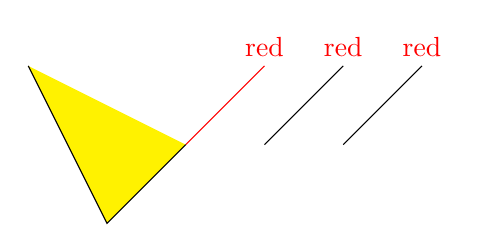
\begin{tikzpicture}
\draw[red]			(0,0) -- +(1,1) node[above]			{red};
\draw[text=red]	(1,0) -- +(1,1) node[above]			{red};
\draw						(2,0) -- +(1,1) node[above,red]	{red};
	\filldraw[fill=yellow] (0,0) -- (-1, -1) -- (-2, 1);
\end{tikzpicture}

%</example-.tex>
% \end{latexcode}
% ^^A ]]] End of subsubsection `tikz'.
%
% \subsubsection{xfig}^^A [[[
% 
% ^^A ]]] End of subsubsection `xfig'.
%
% \subsubsection{xypic}^^A [[[
% The \verb|xypic| package is an older package for creating graphics.
% However, it is more difficult to use and to learn because the syntax and the documentation are
% a bit cryptic\footnote{cryptic: 隠(さ)れた,秘密の,なぞの,意味不明の\mycite[keyword=cryptic]{genius}}
% \texdoc[section=1.2 Comparison with Other Graphics Packages]{tikz}.
% ^^A ]]] End of subsubsection `xypic'.
%
% ^^A ]]] End of subsection `***'.
%
% ^^A ]]] End of section `Graphics関係'.
%
% \section{Table関係}^^A [[[
%
% \subsection{Notes}^^A [[[
% \begin{myitemize}
% \1 \href{https://www.overleaf.com/learn/latex/tables#Multi-page_tables}{Tables (Overleaf)}
% \1 The \verb|xtab| package enables long tables to be automatically broken at page boundaries.
% It is an extension of the \verb|supertabular| package and also reduces or eliminates some of its weaknesses
% \texdoc[section=Abstract]{xtab}
% \1 
% \end{myitemize}
% ^^A ]]] End of subsection `Notes'.
%
% \subsection{各Packageの詳細}^^A [[[
%
% \subsubsection{longtable}^^A [[[
% \begin{myitemize}
% \1 Maintained by the \LaTeX{} Project team
% \1 
% \end{myitemize}
% ^^A ]]] End of subsubssection `longtable'.
%
% \subsubsection{supertabular}^^A [[[
% \begin{myitemize}
% \1 Author: not \LaTeX{} Project team
% \1 
% \end{myitemize}
% ^^A ]]] End of subsubssection `supertabular'.
%
% \subsubsection{xtab}^^A [[[
% \begin{myitemize}
% \1 Author: not \LaTeX{} Project team
% \1 
% \end{myitemize}
%
% \begin{latexcode}
%<*sample-philex.tex>
\documentclass{ltjsarticle}
\usepackage{philex}
\begin{document}
\noindent Eulerの業績:
\lb{label1}{Euler's formula
    \lba{label1-1} $e^{ix}=\cos x+i\sin x$
}
など.
\rf{label1-1}からEulerの等式が得られる.
\end{document}
%</sample-philex.tex>
% \end{latexcode}
% ^^A ]]] End of subsubsection `xtab'.
%
% \subsubsection{}^^A [[[
% \begin{myitemize}
% \1 
% \end{myitemize}
% ^^A ]]] End of subsubssection `'.
%
% ^^A ]]] End of subsection `Package'.
%
%
%
%
%
% ^^A ]]] End of section `Table関係'.
%
% \section{見出し関係}^^A [[[
%
% \subsection{調査したパッケージ}^^A [[[
% 次のパッケージを調べた:
% \begin{myitemize}
% \1 anonchap
%   \2 
% \1 fncychap
%   \2 
% \1 sectsty
%   \2 
% \1 titlesec
%   \2 
% \1 tocbibind
%   \2 
% \end{myitemize}
% ^^A ]]] End of subsection `***'.
%
% \subsection{関連パッケージについて比較・言及されている記事}^^A [[[
% \begin{myitemize}
% \1 \href{https://texfaq.org/FAQ-secthead}{ここ}にまとめられている
% \1 \texdoc[section=1. Introduction]{titlesec}
% \1 
% \end{myitemize}
% ^^A ]]] End of subsection `***'.
%
% \subsection{各パッケージについて}^^A [[[
%
% \subsubsection{}^^A [[[
%
%    \begin{macrocode}
%<*example-.tex>




%</example-.tex>
%    \end{macrocode}
% ^^A ]]] End of subsubsection `'.
%
% \subsubsection{}^^A [[[
%
%    \begin{macrocode}
%<*example-.tex>




%</example-.tex>
%    \end{macrocode}
% ^^A ]]] End of subsubsection `'.
%
% ^^A ]]] End of subsection `***'.
%
% ^^A ]]] End of section `見出し関係'.
%
% \section{Defining new command関係}^^A [[[
% タイトルはテキトーにつけた
%
% \subsection{関連パッケージについて比較・言及されている記事}^^A [[[
% \begin{myitemize}
% \1 
% \1 
% \end{myitemize}
% ^^A ]]] End of subsection `***'.
%
% \subsection{各パッケージについて}^^A [[[
%
% \subsubsection{etoolbox}^^A [[[
%
%    \begin{macrocode}
%<*example-.tex>




%</example-.tex>
%    \end{macrocode}
% ^^A ]]] End of subsubsection `'.
%
% \subsubsection{newcommand}^^A [[[
%
%    \begin{macrocode}
%<*example-.tex>




%</example-.tex>
%    \end{macrocode}
% ^^A ]]] End of subsubsection `'.
%
% \subsubsection{xargs}^^A [[[
%
%    \begin{macrocode}
%<*example-.tex>




%</example-.tex>
%    \end{macrocode}
% ^^A ]]] End of subsubsection `xargs'.
%
% \subsubsection{xparse}^^A [[[
% \begin{myitemize}
% \1 Abstract
% \1 Author
%   \2 The \LaTeX3 Project
% \1 Conclusion
% \end{myitemize}
%
% 基本形な使い方\texdoc[section=2 Declaring commands and environments]{xparse}:
%
% \verb|\NewDocumentCommand <function> {<arg spec>} {<code>}|
%
% \verb|\NewDocumentEnvironment {<environment>} {<arg spec>} {<start code>} {<end code>}|
%
%
%
%
%
%
%
%
%
% \href{https://qiita.com/zr_tex8r/items/50168ad7087516c3e139}{ここ}で詳しく説明がなされている.
%
% オプション引数の指定\verb|O|は必ず「既定値の指定」をもち、省略した時の動作は
% 「既定値を指定したときと同じ」でした。
% これに対して、「引数が指定されたか否かで条件分岐したい」という場合が考えられます。
% 例えば、先の例の\verb|\myAlertA[色名]{テキスト}|について、
% 「色名が省略された場合は特定の“既定の色”にするのでなく、そもそも色変更を行わない」
% という動作に変えたいとします。
% この命令を\verb|\myAlertD|とすると、この命令の動作は次のようになるべきで、
% どうしても条件分岐が必要となってきます。
% \begin{myitemize}
% \1 \verb|\myAlertD[red]{アレ}| → \verb|{\color{red}\Large アレ}|
% \1 \verb|\myAlertD{アレ}| → \verb|{\Large アレ}|
% \end{myitemize}
% これを実現するには、「既定値なしのオプション引数」を表す引数仕様文字である
% 小文字の\verb|o|(optional)を利用します。

%    \begin{macrocode}
%<*example-xparse-1.tex>
\NewDocumentCommand\myAlertD{o m}{%
% #1=色名(省略可), #2=テキスト
  {%
    \IfValueT{#1}{\color{#1}}%
    \Large #2%
  }%
}



%</example-xparse-1.tex>
%    \end{macrocode}
% ^^A ]]] End of subsubsection `xparse'.
%
% \subsubsection{}^^A [[[
%
%    \begin{macrocode}
%<*example-.tex>




%</example-.tex>
%    \end{macrocode}
% ^^A ]]] End of subsubsection `'.
%
% ^^A ]]] End of subsection `***'.
%
% ^^A ]]] End of section `Defining new command関係'.
%
% \section{Key-value interfaces???}^^A [[[
% タイトルは\texdoc[section=Part XXI The l3keys package]{l3keys}より.
%
% \subsection{調査したパッケージ}^^A [[[
% 次のパッケージを調べた:
% \begin{myitemize}
% \1 l3keys(2e)
% \1 keyreader
%   \2 The package provides a robust interface to controlling keys in xkeyval,
%   removing some of that package's restrictions.
% \1 keyval
% \1 kvoptions
%   \2 Supports keyval processing of package/class options.
% \1 kvsetkeys
% \1 pgfkeys
%   \2 part of PGF/TikZ
% \1 pgfkeyx
% \1 pgfopts
%   \2 Allows pgfkeys processing to be performed on class or package options.
% \1 scrbase
% \1 xkeyval
% \1 ...
% \1 \href{https://tex.stackexchange.com/questions/26771/a-big-list-of-every-keyval-package}{参照先1}にまだまだ載ってる.
% \end{myitemize}
% ^^A ]]] End of subsection `***'.
%
% \subsection{関連パッケージについて比較・言及されている記事}^^A [[[
% \begin{myitemize}
% \1 \href{https://tex.stackexchange.com/questions/26771/a-big-list-of-every-keyval-package}{参照先1}
% \1 \href{http://www.tug.org/tugboat/tb30-1/tb94wright-keyval.pdf}{参照先2}
% \1 \texdoc[section=12 Additional packages]{xkeyval}
% \1 \texdoc[section=82.1.1]{pgfkeys}
% \1 \texdoc[section=82 Key Management]{pgfkeys}
% \end{myitemize}
% ^^A ]]] End of subsection `***'.
%
% \subsection{各パッケージについて}^^A [[[
%
% \subsubsection{l3keys}^^A [[[
% The \LaTeX3 Project
% \begin{myitemize}
% \1 part of expl3
%   \2 expl3とは\LaTeX3チームが開発しているプログラミング言語
%   \urlref{https://blog.wtsnjp.com/2017/10/29/intro-expl3/}{LaTeX3}
% \1 Inspired by pgfkeys.
% \1 Use l3keys2e to use it in options of \LaTeXe\ packages and classes.
% \1 \verb|\ExplSyntaxOn <code> \ExplSyntaxOff|
%   \2 The \verb|\ExplSyntaxOn| function switches to a category code régime in which spaces are ignored
%   and in which the colon (\verb|:|) and underscore (\verb|_|) are treated as \doublequotes{letters},
%   thus allowing access to the names of code functions and variables.
%   Within this environment, \verb|~| is used to input a space.
%   The \verb|\ExplSyntaxOff| reverts to the document category code régime
%   \texdoc[part=II, section=1 Using the \LaTeX3 modules]{interface3}.
%   \2 \urlref{https://tex.stackexchange.com/questions/108696/what-do-explsyntaxon-and-explsyntaxoff-do}{ExplSyntaxOn}
% \1 \verb|\group_begin:|, \verb|\group_end:|
%   \2 These functions begin and end a group for definition purposes.
%   Assignments are local to groups unless carried out in a global manner.
%   (A small number of exceptions to this rule will be noted as necessary elsewhere in this document.)
%   Each \verb|\group_begin:| must be matched by a \verb|\group_end:|,
%   although this does not have to occur within the same function.
%   Indeed, it is often necessary to start a group within one function and finish it within another,
%   for example when seeking to use non-standard category codes
%   \texdoc[part=IV, section=2 Grouping material]{interface3}
% \1 \verb|xparse|パッケージ内部で\verb|expl3|パッケージを読み込んでいる
%   \2 \href{/usr/share/texlive/texmf-dist/tex/latex/l3packages/xparse/xparse.sty}{xparse.sty}
% \1 \verb|expl3|パッケージ内部で\verb|l3keys|パッケージを読み込んでいる?????
% \1 
% \1 
% \end{myitemize}
%
% \paragraph{Example 1}^^A [[[
% \verb|example-l3keys-1.tex|は「output:sample????????」と出力される.
%    \begin{macrocode}
%<*example-l3keys-1.tex>
\documentclass{ltjsarticle}
\usepackage{xparse}
\ExplSyntaxOn
\keys_define:nn { mymodule }{%
    key .code:n = #1
}
\NewDocumentCommand \mycommand { o m }{%
    % \group_begin:
    \keys_set:nn { mymodule }{ #1 }
    % \group_end:
}
\ExplSyntaxOff
\begin{document}
\mycommand{key=sample}
\end{document}
%</example-l3keys-1.tex>
%    \end{macrocode}
% ^^A ]]] End of paragraph `Example 1'.
%
% \paragraph{Example 2}^^A [[[
% \verb|example-l3keys-2.tex|は「output:sample,output:\textbf{*initial*}?????」となる.
%    \begin{macrocode}
%<*example-l3keys-2.tex>
\documentclass{ltjsarticle}
\usepackage{expl3,xparse}
\ExplSyntaxOn
\keys_define:nn { mymodule }{%
    key .code:n     =output:#1,
    key .default:n  = \textbf{*initial*}
}
\NewDocumentCommand \mycommand { m }{%
    \group_begin:
    \keys_set:nn { mymodule }{ #1 }
    \group_end:
}
\ExplSyntaxOff
\begin{document}
\mycommand{key=sample},
\mycommand{key}
\end{document}
%</example-l3keys-2.tex>
%    \end{macrocode}
% ^^A ]]] End of paragraph `Example 2'.
%
% \paragraph{Example 3}^^A [[[
% \verb|example-l3keys-3.tex|は
% 「\texttt{sample}, (Euler)\texttt{test}, (Einstein)-Dedekind-\texttt{argument}」となる.
%
%    \begin{macrocode}
%<*example-l3keys-3.tex>
\documentclass{ltjsarticle}
\usepackage{expl3,xparse}
\ExplSyntaxOn
\keys_define:nn { mymodule }{%
    key-one .code:n =(#1),
    key-two .code:n =-#1-
}
\DeclareDocumentCommand \MyModuleMacro { O{} m }{%
    \group_begin:
    \keys_set:nn { mymodule } { #1 }
    \texttt{#2}
    \group_end:
}
\ExplSyntaxOff
\begin{document}
\MyModuleMacro{sample},
\MyModuleMacro[key-one=Euler]{test},
\MyModuleMacro[key-one=Einstein,key-two=Dedekind]{argument}
\end{document}
%</example-l3keys-3.tex>
%    \end{macrocode}
% ^^A ]]] End of paragraph `Example 3'.
%
% \paragraph{Example 4}^^A [[[
% \verb|example-l3keys-4.tex|
%
%    \begin{macrocode}
%<*example-l3keys-4.tex>
\documentclass{ltjsarticle}
\usepackage{expl3,tcolorbox,xparse}
%
\newenvironment{test}{%
    \tcolorbox
}{%
    \endtcolorbox
}
%
\ExplSyntaxOn
\RenewDocumentCommand \test { O{} O{} }{%
    \tcolorbox[#1,#2]
}
\ExplSyntaxOff
%
\begin{document}
\begin{test}
sample
\end{test}

\begin{test}[title=This is a test.][colframe=blue]
\LaTeX
\end{test}
\end{document}
%</example-l3keys-4.tex>
%    \end{macrocode}
% ^^A ]]] End of paragraph `Example 4'.
%
% \paragraph{Example }^^A [[[
% \verb|example-l3keys-.tex|は「\texttt{sample} (test)\texttt{argument}」となる.
%
%    \begin{macrocode}
%<*example-l3keys-.tex>
%</example-l3keys-.tex>
%    \end{macrocode}
% ^^A ]]] End of paragraph `Example '.
%
% \paragraph{Example }^^A [[[
% \verb|example-l3keys-.tex|は「\texttt{sample} (test)\texttt{argument}」となる.
%
%    \begin{macrocode}
%<*example-l3keys-.tex>
%</example-l3keys-.tex>
%    \end{macrocode}
% ^^A ]]] End of paragraph `Example '.
%
%
%
% ^^A ]]] End of subsubsection `'.
%
% \subsubsection{xkeyval}^^A [[[
% \verb|xkeyval|の説明が\url{https://en.wikibooks.org/wiki/LaTeX/Macros#Extending_the_number_of_arguments}にある.
%
%
%
% \verb|example-xkeyval-1.tex|は「これはテストです.」となる.
%
%    \begin{macrocode}^^A [[[
%<*example-xkeyval-1.tex>
\documentclass{ltjsarticle}
\usepackage{xkeyval}
\makeatletter
\define@key{sample}{keytest}{これはテストです.}
\makeatother
\begin{document}
\makeatletter
\KV@sample@keytest
\makeatother
\end{document}
%</example-xkeyval-1.tex>
%    \end{macrocode}^^A ]]]
%
% \verb|example-xkeyval-2.tex|は「これは別のテストです.」となる.
%
%    \begin{macrocode}^^A [[[
%<*example-xkeyval-2.tex>
\documentclass{ltjsarticle}
\usepackage{xkeyval}
\makeatletter
\define@key{sample}{keytest}{これは#1です.}
\makeatother
\begin{document}
\makeatletter
\KV@sample@keytest{別のテスト}
\makeatother
\end{document}
%</example-xkeyval-2.tex>
%    \end{macrocode}^^A ]]]
%
% \verb|example-xkeyval-3.tex|は以下のようになる.
%
% baseball
%
% soccersoccer
%
% baseballbaseball
%
%    \begin{macrocode}^^A [[[
%<*example-xkeyval-3.tex>
\documentclass{ltjsarticle}
\usepackage{xkeyval}
\makeatletter
\define@key{example}{key}{baseball}
\define@key{sample}{key}{soccer}
\makeatother
\newcommand{\example}[1]{\setkeys{example}{#1}}
\newcommand{\sample}[1]{\setkeys{sample}{#1}}
\begin{document}
\example{key=4321}
\sample{key=TeX,key=090}
\example{key=LaTeX,key=Vim}
\end{document}
%</example-xkeyval-3.tex>
%    \end{macrocode}^^A ]]]
%
% \verb|example-xkeyval-4.tex|は以下のようになる.
%
% 4321
%
% テスト13579
%
% ECE42
%
%    \begin{macrocode}^^A [[[
%<*example-xkeyval-4.tex>
\documentclass{ltjsarticle}
\usepackage{xkeyval}
\makeatletter
\define@key{example}{key1}{#1}
\define@key{example}{key2}{テスト}
\makeatother
\newcommand{\example}[1]{\setkeys{example}{#1}}
\begin{document}
\example{key1=4321}

\example{key2=ABC,key1=13579}

\example{key1=ECE,key1=42}
\end{document}
%</example-xkeyval-4.tex>
%    \end{macrocode}^^A ]]]
%
% \verb|example-xkeyval-5.tex|は以下のようになる.
%
% これはテストです.
%
% これは別のテストです.
%
%    \begin{macrocode}^^A [[[
%<*example-xkeyval-5.tex>
\documentclass{ltjsarticle}
\usepackage{xkeyval}
\makeatletter
\define@key{sample}{key}[テスト]{これは#1です.}
\makeatother
\newcommand{\sample}[1]{\setkeys{sample}{#1}}
\begin{document}
\sample{key}

\sample{key=別のテスト}
\end{document}
%</example-xkeyval-5.tex>
%    \end{macrocode}^^A ]]]
%
% \verb|example-xkeyval-6.tex|は以下のようになる.
%
% これはテストです.
%
% これは別のテストです.
%
%    \begin{macrocode}^^A [[[
%<*example-xkeyval-6.tex>
\documentclass{ltjsarticle}
\usepackage{xkeyval}
\makeatletter
\define@key{sample}{key}[テスト]{これは#1です.}
\makeatother
\newcommand{\sample}[1][key]{\setkeys{sample}{#1}}
\begin{document}
\sample

\sample[key=別のテスト]
\end{document}
%</example-xkeyval-6.tex>
%    \end{macrocode}^^A ]]]
%
% 以下クラスオプションへの適用例を示す.
%
% \texdoc[section=7 Package option processing]{xkeyval}の\verb|\DeclareOptionX|の箇所にある例を参考にした.
%
%    \begin{macrocode}^^A [[[
%<*example-xkeyval-cls.tex>
\LoadClass{ltjsarticle}
\RequirePackage{xkeyval}
\DeclareOptionX{parindent}[5pt]{\setlength\parindent{#1}}
\ProcessOptionsX\relax
\ProcessOptions\relax
%</example-xkeyval-cls.tex>
%    \end{macrocode}^^A ]]]
%
%    \begin{macrocode}^^A [[[
%<*example-xkeyval-7.tex>
\documentclass[parindent=30pt]{example-xkeyval-cls}
\begin{document}
This is \LaTeX test.
\end{document}
%</example-xkeyval-7.tex>
%    \end{macrocode}^^A ]]]
%
% ^^A ]]] End of subsubsection `xkeyval'.
%
% ^^A ]]] End of subsection `***'.
%
% ^^A ]]] End of section `Key-value'.
%
% \section{Index関係}^^A [[[
%
%
% \subsection{各Packageの詳細}^^A [[[
%
% \subsubsection{ltxindex}^^A [[[
%
%
%
% ^^A ]]] End of subsubsection `ltxindex'.
%
% \subsubsection{makeindex}^^A [[[
%
%
%
% ^^A ]]] End of subsubsection `makeindex'.
%
% ^^A ]]] End of subsection `Package'.
%
%
%
% ^^A ]]] End of section `Index関係'.
%
% \section{Font関係}^^A [[[
%
%
% \subsection{各Packageの詳細}^^A [[[
%
% \subsubsection{libertine}^^A [[[
% \texdoc{scontents}を見て気に入ったフォント.
%
%
%
% ^^A ]]] End of subsubsection `libertine'.
%
% ^^A ]]] End of subsection `Package'.
%
%
%
% ^^A ]]] End of section `Font関係'.
%
% \section{記号関係}^^A [[[
% \texdoc{symbols-a4}でたくさんの記号がまとめられたものが見れる.
%
%
% \subsection{各Packageの詳細}^^A [[[
%
% \subsubsection{pifont}^^A [[[
% 
%
%
%
%
% ^^A ]]] End of subsubsection `pifont'.
%
% \subsubsection{textcomp}^^A [[[
% 
%
%
%
%
% ^^A ]]] End of subsubsection `textcomp'.
%
% ^^A ]]] End of subsection `Package'.
%
%
% ^^A ]]] End of section `記号関係'.
%
% ^^A End of file `notes.tex'.
